\documentclass[twocolumn, a4paper]{UECIEresume}

\usepackage[dvipdfmx]{graphicx}
\usepackage{graphicx}
\usepackage{amsmath}
\usepackage{txfonts}
\usepackage{url}
\usepackage{enumerate}

\setlength\intextsep{0pt}
\setlength\textfloatsep{0pt}


\title{複数人で使用可能な3Dアイデアノートシステムの提案と実装}
\date{平成 29 年 9 月 26 日}
\affiliation{情報学専攻 メディア情報学プログラム}
\supervisor{田野 俊一 教授,橋山 智訓 准教授}
\studentid{1630012}
\author{猪膝 孝之}
%\headtitle{平成 yy 年度 総合情報学科 卒業論文中間発表}
%\headtitle{平成 yy 年度 総合情報学科 卒業論文発表}
%\headtitle{平成 29 年度 情報学専攻 修士論文中間発表}
\headtitle{平成 29 年度 情報学専攻 修士論文発表}



\begin{document}
\maketitle

\section{はじめに}
近年、HMD(Head Mounted Display)が普及してきた。現在、HMD に関する多くの研究は一人で使うことが想定されている。また、特定の場所において使用することを想定している場合も多い。そして、手やペンで描くのみで入力手法が限定されている場合も多い。現状では複数人で使用することを想定していたり、外などの広い空間で利用することを想定していたり、手で描くだけでなく音声でも入力可能なシステムを想定している研究やアプリケーションは少ない。そこで、複数人で使用できて、どこでも利用できて、様々な入力ができるシステムが必要だと考え、本研究の立案に至った。

\section{従来研究と問題点}
椎尾ら\cite{tex1,tex2}は仮想の手書きメモによるコミュニケーションをウェアラブルコンピュータにより実現する空気ペンを試作した。問題点としては、同時に複数人で使用できないことや、使用できる範囲がRFIDタグがついた床上のみなので場所が限定されることが挙げられる。

また、高山ら\cite{tex3,tex4}は実世界のどのような時間・場所であっても、ユーザが思い浮かんだふとしたアイデアを、生起を誘発したコンテキストに対応づけて保存し、それを他のユーザと共有できるシステムを作成した。問題点としては、多くの機器を装着しなければならないので持ち運びが大変であることや、操作が複雑なので慣れるのに時間がかかることが挙げられる。

長田ら\cite{tex5}はスマートグラスを用いた仮想空間への手書き情報共有システムを提案した。問題点としては、指のみの操作だとできることが限定されることが挙げられる。

従来研究の問題点をまとめると以下である。

\begin{itemize}
 \item HMDを付けて同時に複数人で使用することを想定していない
 \item HMDを付けて使用するシステムで利用できる場所が限定されている
 \item HMDを付けて使用するシステムで入力手法が限定されている
\end{itemize}


\section{本研究のコンセプト}
従来研究ではHMD を付けて同時に複数人で使用することを想定していない、HMD を付けて使用するシステムで利用できる場所が限定されている、HMD を付けて使用するシステムで入力手法が限定されているという問題点があった。そこで、本研究は以下の三つを満たすようなHMDを使用したシステムを提案する。
\begin{enumerate}[(1)]
 \item 複数人で同時に使用することが可能
 \item どこでも場所を選ばず利用が可能
 \item 簡単な操作で直感的で様々な入力が可能
\end{enumerate}

\section{システム設計}
ハードウェアは可搬性を考慮して、マイクロソフト社のHoloLens\cite{hololens}を使用する。

\subsection{全体設計}
本研究のコンセプトで述べた(1)、(2)、(3)を踏まえると、システムとして必要な機能は大きく分けて、メモを入力、メモを操作、メモを共有の三つである。以下にそれぞれについて詳細を述べる。

\subsection{メモを入力}
実世界の任意の3D空間上に図形や文字のメモを描いて残したり話して残したりできるようにする。3D空間上に文字によるメモを相手に見えるようにするためには回転して相手に向けるという手法が考えられる。しかし、平面に残したメモの場合、その面自体に意味があるので回転させてはならない。そこで、正面からメモを見た場合はそのまま表示し、ある程度横から見た場合にはそのメモ自体はそのままだが、内容がわかるように目の前に見やすく表示をするという手法を提案する。(図\ref{fig:memo_wall})

\begin{figure}[h]
  \begin{center}
    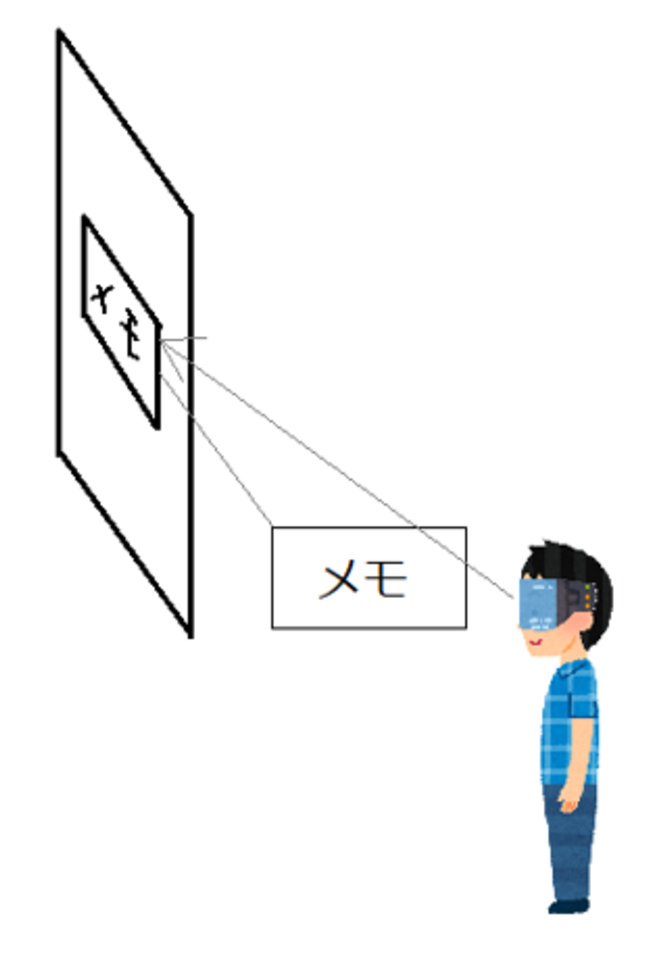
\includegraphics[clip,height=6.0cm,width=4.0cm]{./memo_wall.eps}
    \caption{ある程度横から見た場合は目の前にも表示}
    \label{fig:memo_wall}
  \end{center}
\end{figure}


\subsection{メモを操作}
広い空間上にメモを残す場合、遠くに配置してあるメモをどうやって選択、移動、削除するかという問題が発生する。そこで、以下の三つのインタラクションを提案する。

\begin{enumerate}[(1)]
 \item ルームスケールチェンジ
 \item 3Dラバーバンド
 \item 3Dフィッシング
\end{enumerate}

(1)手元に部屋全体を縮小したものを用意してメモを操作する手法で、(2)はイメージとしては手元に輪ゴムがついたオブジェクトを引っ張って遠隔のメモを操作する手法、(3)は視線と手元のオブジェクトを利用して釣りのように遠隔のメモを操作する手法である。

\subsection{メモを共有}
実世界の任意の3D空間上に残したメモを対面にいる人だけでなく、遠隔にいる人にもメモを共有できるようにする。遠隔にいる人はアバターを実世界に表示させる。

\section{プロトタイプシステムの実装}
ハードウェアはHoloLensを利用し、開発環境はWindows10でUnity\cite{unity}を使用した。実装したアプリケーションをHoloLensにインストールした。HoloToolkit\cite{holotoolkit}のSharingという機能を利用し、Sharing用のサーバを介して空間の共有を行った。また、ユーザが喋った内容をテキストに変換するクラウドサービスであるGoogle Cloud Speech API\cite{speech}を利用した。

\section{プロトタイプの評価実験}
実装したプロトタイプシステムの評価実験を行った。本実験ではまず決められた手順に従って被験者に操作をしてもらうシナリオ実験と被験者自ら考えて操作を行って課題を解決する課題解決実験で構成される。被験者は男女10人で平均年齢23.7歳である。実験は被験者2人で1グループとして同時に行った。

\subsection{実験結果}
シナリオ実験での手順の遂行状況においてはほとんどの手順において成功率100\%という結果になった。課題解決実験のほうに関してもほとんどの被験者が自ら考えてプロトタイプシステムを利用してタスクを実行できることがわかった。また、実験後のアンケート結果では、プロトタイプシステムの機能によっては好みが分かれるものあったが、全体的な評価は高かった。

\section{まとめ}
本研究では複数人で使用できて、どこでも利用できて、直感的で様々な入力ができるHMDを使用したシステムの提案と実装を行った。プロトタイプシステムの評価実験の結果より、被験者はこのシステムを利用して3D空間上にメモを残して共有できることが確認できた。今後の課題としてはシステムの各機能の改善と共有機能の改善等が挙げられる。

\vspace{-1zh}

{\small
\begin{thebibliography}{99}
\bibitem{tex1}
        山本, 椎尾:
        空気ペン―空間への描画による情報共有-;
        情報処理学会全国大会講演論文集,
        {\bf Vol.59}, No.4, pp.39-40(1999).
\bibitem{tex2}
	椎尾, 山本:
	コミュニケーションツールのための簡易型ARシステム;
	コンピュータソフトウェア, 
        {\bf Vol.19}, No.4, pp.246-253(2002).
\bibitem{tex3}
	高山, 瑞慶山, 田野, 岩田, 橋山:
	実世界コンテキスト・情報を用いたユビキタスインフォーマルコミュニケーションの実装と評価;
	ヒューマンインタフェースシンポジウム2005,
        pp.955-958(2005).
\bibitem{tex4}
        Tano, S., Takayama, T., Iwata, M. and Hashiyama, T.:
        Wearable Computer for Ubiquitous Informal Communication;
        Sixth International Workshop on Smart Appliances and Wearable Computing-IWSAWC 2006-(at 26th IEEE International Conference on Distributed Computing Systems ICDCS),
        pp.1-8(2006).
\bibitem{tex5}
        長田, 佐々木, 島田, 佐藤:
        スマートグラスを用いた仮想空間への手書き情報共有システム;
        情報処理学会第77回全国大会論文集,
        3-205, 206(2015).
\bibitem{hololens}
        Microsoft Inc:
        HoloLens;
        \textless\url{https://www.microsoft.com/ja-jp/hololens}\textgreater2018年2月1日アクセス.
\bibitem{unity}
        Unity Technologies Inc:
        Unity;
        \textless\url{https://unity3d.com/jp/unity}\textgreater2018年2月1日アクセス.
\bibitem{holotoolkit}
        Microsoft Inc:
        HoloToolkit;
        \textless\url{https://github.com/Microsoft/HoloToolkit-Unity}\textgreater2018年2月1日アクセス.
\bibitem{speech}
	Google Inc.:
	Google Cloud Speech API;
	\textless\url{https://cloud.google.com/speech/?hl=ja}\textgreater2018年2月1日アクセス.
\end{thebibliography}
}
\end{document}